\documentclass{zc-ust-hw}

\usepackage[backend=biber, style=ieee]{biblatex}
\addbibresource{references.bib}

\usetikzlibrary{chains}
\usepackage{./tikz-dsp}
\DeclareMathAlphabet{\mathpzc}{OT1}{pzc}{m}{it}
\newcommand{\z}{\mathpzc{z}}

\name{SalahDin Ahmed Salh Rezk}
\id{202201079}
\course{Signals and Systems (CIE 227)}
\assignment{Assignment 3}

\begin{document}

\maketitle
\vspace*{-2.5em}
\tableofcontents
\listoffigures

\newpage

\section{Introduction to FIR Filters}

\subsection{Concept} An FIR filter is a type of digital filter used in
signal processing. It operates on a discrete-time signal i.e. it
processes data that is sampled at specific intervals. The core idea
behind FIR filters is to perform convolution between the input signal
and a set of filter coefficients (also known as taps). These
coefficients determine how the filter processes the input signal to
achieve desired filtering characteristics.

\subsection{Characteristics}
\begin{enumerate}
  \item \textbf{Finite Impulse Response:} The term "finite" indicates
    that the filter's output response to an impulse (a single sample of
    unity magnitude followed by zeros) is of finite duration. This
    makes FIR filters inherently stable and easy to implement in
    digital systems.
  \item \textbf{Linear Phase Response:} FIR filters can achieve linear
    phase response, meaning they introduce constant delay across all
    frequencies. This characteristic is desirable in applications where
    phase distortion must be minimized, such as in audio processing.
  \item \textbf{Finite Impulse Response:} As the name suggests, FIR
    filters have a finite impulse response, which means that their
    output response to an impulse input eventually decays to zero.
  \item \textbf{No Feedback:} Unlike IIR (Infinite Impulse Response)
    filters, FIR filters do not have feedback loops in their structure.
    This absence of feedback simplifies their implementation and
    eliminates stability concerns related to feedback loops.
\end{enumerate}
\subsection{Applications}
\begin{enumerate}
  \item \textbf{Digital Signal Processing:} FIR filters are widely used
    in digital signal processing applications such as audio processing,
    image processing, communication systems, biomedical signal
    processing, and more.
  \item \textbf{Audio Processing:} FIR filters are used in audio
    equalization, noise reduction, and echo cancellation. \cite{pawar2014design}
  \item \textbf{Image Processing:} FIR filters are used in image
    enhancement, edge detection, and image restoration. \cite{lab6_manual}
  \item \textbf{Communication Systems:} FIR filters are used in
    channel equalization, pulse shaping, and digital modulation. \cite{hossain2021review}
  \item \textbf{Biomedical Signal Processing:} FIR filters are used in
    ECG signal processing, EEG signal analysis, and medical imaging. \cite{marchon2019efficient}
\end{enumerate}
\subsection{Structure}
The basic structure of an FIR filter consists
of input samples, filter coefficients (taps), and a summing junction.
It operates by convolving the input signal with the filter coefficients
to produce the filtered output signal.
\begin{enumerate}
  \item \textbf{Input Signal ($x[n]$):} The input to an FIR filter is a
    sequence of discrete-time samples, where \(n\) represents the time
    index.
  \item \textbf{Filter Coefficients ($h[n]$):} The filter coefficients
    are the weights applied to the input samples during convolution.
    These coefficients determine the filter's frequency response and
    filtering characteristics.
  \item \textbf{Convolution Operation (\(*\)):} The convolution operation
    involves multiplying the input samples by the filter coefficients
    and summing the results to produce the output signal.
  \item \textbf{Summing Junction (\(\sum\)):} The summing junction
    weighted input samples to generate the output signal.
  \item \textbf{Output Signal ($y[n]$):} The output of an FIR filter is
    the result of convolving the input signal with the filter
    coefficients. It represents the filtered version of the input
    signal.
\end{enumerate}
\begin{equation}
  y[n] = \sum_{k=0}^{N-1} h[k] * x[n-k]
\end{equation}
The sum runs over the range of filter coefficients from $k=0$ to
$N-1$, where $N$ is the number of taps or coefficients in the FIR
filter.

The filter coefficients $h[k]$ are typically designed based on the
desired frequency response of the filter, such as low-pass, high-pass,
band-pass, or notch filters. The order of the FIR filter (determined by
$N$) affects its frequency selectivity and performance characteristics.
\begin{figure}[htbp]
  \centering
  \begin{tikzpicture}

          % Place nodes using a matrix
          \matrix (m1) [row sep=2.5mm, column sep=5mm]
          {
                  %--------------------------------------------------------------------
                  \node[dspnodeopen,dsp/label=above] (m00) {$x[n]$};    &
                  \node[coordinate]                  (m01) {};          &
                  \node[dspnodefull]                 (m02) {};          &
                  \node[coordinate]                   (m03) {}; &
                  \node[dspnodefull]                 (m04) {};          &
                  \node[coordinate]                   (m05) {}; &
                  \node[dspnodefull]                 (m06) {};          &
                  \node[coordinate]                   (m07) {}; &
                  \node[coordinate]                  (m08) {};          &
                  \node[coordinate]                  (m09) {};          &
                  \node[coordinate]                  (m0X) {};          \\
                  %--------------------------------------------------------------------
                  \node[coordinate]                  (m10) {};          &
                  \node[coordinate]                  (m11) {};          &
                  \node[dspmixer, dsp/label=right]   (m12) {$h[0]$};    &
                  \node[coordinate]                  (m13) {};          &
                  \node[dspmixer, dsp/label=right]   (m14) {$h[1]$};    &
                  \node[coordinate]                  (m15) {};          &
                  \node[dspmixer, dsp/label=right]   (m16) {$h[2]$};    &
                  \node[coordinate]                  (m17) {};          &
                  \node[dspmixer, dsp/label=right]   (m18) {$h[3]$};    &
                  \node[coordinate]                  (m19) {};          &
                  \node[coordinate]                  (m1X) {};          \\
                  %--------------------------------------------------------------------
                  \\
                  %--------------------------------------------------------------------
                  \node[coordinate]                  (m20) {};          &
                  \node[coordinate]                  (m21) {};          &
                  \node[coordinate]                  (m22) {};          &
                  \node[coordinate]                  (m23) {};          &
                  \node[dspadder]                    (m24) {};          &
                  \node[coordinate]                  (m25) {};          &
                  \node[dspadder]                    (m26) {};          &
                  \node[coordinate]                  (m27) {};          &
                  \node[dspadder]                    (m28) {};          &
                  \node[coordinate]                  (m29) {};          &
                  \node[dspnodeopen,dsp/label=above] (m2X) {$y[n]$};    \\
                  %--------------------------------------------------------------------
          };

          % Draw connections
          
          \begin{scope}[start chain]
                  \chainin (m00);
                  \chainin (m02) [join=by dspflow];
                  \chainin (m12) [join=by dspconn];
                  \chainin (m22) [join=by dspline];
          \end{scope}

          \foreach \i [evaluate = \i as \j using int(\i+1),
                       evaluate = \i as \k using int(\i+2),] in {2,4,6}
          {
                  \begin{scope}[start chain]
                          \chainin (m0\i);
                          \chainin (m0\j) [join=by dspconn];
                          \chainin (m0\k) [join=by dspline];
                          \chainin (m1\k) [join=by dspconn];
                          \chainin (m2\k) [join=by dspconn];
                  \end{scope}
                  \draw[dspconn] (m2\i) -- (m2\k);
          }

          \draw[dspflow] (m28) -- (m2X);
  \end{tikzpicture}
  \caption{Basic Structure of an FIR Filter}
\end{figure}

\section{Designing a Low-pass FIR Filter}

\subsection{Concept} A low-pass FIR filter is designed to pass signals with
frequencies lower than a specified cutoff frequency while attenuating signals
with higher frequencies. This type of filter is commonly used in applications
where high-frequency noise or interference must be removed while preserving the
low-frequency components of the signal.
  
\subsection{Design Steps:}
\begin{enumerate}
  \item \textbf{Determine Specifications:} Specify the desired cutoff
    frequency, passband ripple, stopband attenuation, and filter order.
  \item \textbf{Design Filter Coefficients:} Use windowing, frequency
    sampling, or optimization techniques to design the filter
    coefficients based on the desired frequency response.
  \item \textbf{Implement Filter:} Implement the FIR filter using the
    designed coefficients and convolve it with the input signal to
    obtain the filtered output.
\end{enumerate}

\newpage
\subsection{MATLAB Code}
\begin{minted}[
  frame=single,
  bgcolor=gray!10!white,
  linenos,
]{matlab}
Fs = 8000;      % Sampling frequency in Hz
Fc = 1000;      % Cutoff frequency in Hz
N = 50;         % Filter order
ftype = "low";  % Filter type

Fc_norm = Fc / (Fs/2);        % Normalize the cutoff frequency
h = fir1(N, Fc_norm, ftype);  % Design the filter

freqz(h, 1, 1024, Fs); % Plot the frequency response of the filter
\end{minted}
In this code snippet, the \texttt{fir1} function is used to design an
FIR filter with a low-pass response. The filter order \texttt{N}, cutoff
frequency \texttt{Fc}, and sampling frequency \texttt{Fs} are specified
to design the filter coefficients \texttt{h}. The frequency response of
the filter is then plotted using the \texttt{freqz} function.
    
\begin{figure}[htbp]
  \centering
  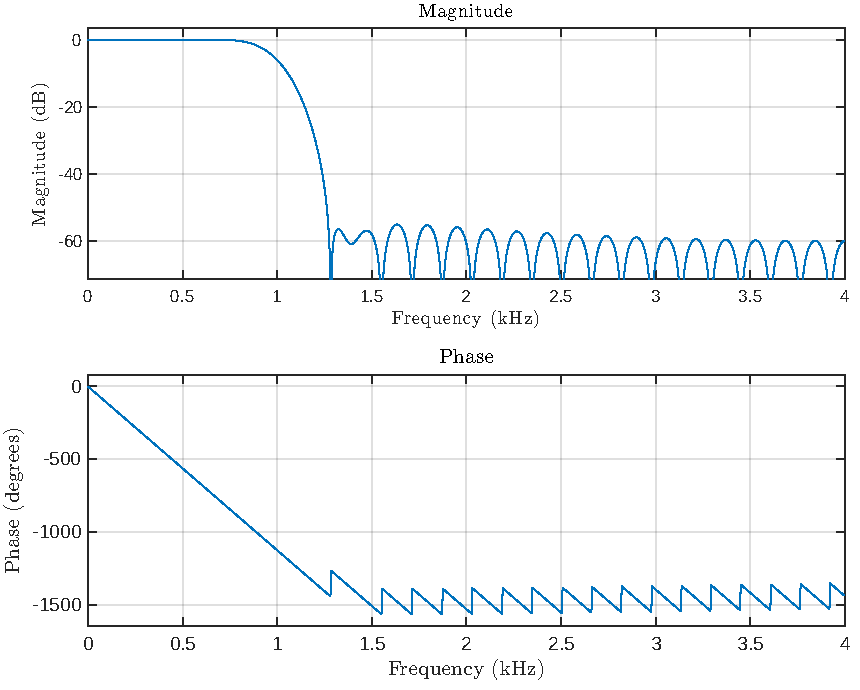
\includegraphics[width=0.75\textwidth]{figures/low-pass-fir-filter.pdf}
  \caption{Frequency Response of FIR Low-Pass Filter}
\end{figure}

\subsection{Frequency Response:} The frequency response of a low-pass
FIR filter shows the attenuation of high-frequency components beyond the
cutoff frequency. The passband region contains the low-frequency
components that are passed by the filter, while the stopband region
shows the attenuation of high-frequency components.

\section{Designing a High-pass FIR Filter}

\subsection{Concept} A high-pass FIR filter is designed to pass signals with
frequencies higher than a specified cutoff frequency while attenuating signals
with lower frequencies. This type of filter is commonly used in applications
where low-frequency noise or interference must be removed while preserving the
high-frequency components of the signal.

\subsection{Design Steps}
\begin{enumerate}
  \item \textbf{Determine Specifications:} Specify the desired cutoff
    frequency, passband ripple, stopband attenuation, and filter order.
  \item \textbf{Design Filter Coefficients:} Use windowing, frequency
    sampling, or optimization techniques to design the filter
    coefficients based on the desired frequency response.
  \item \textbf{Implement Filter:} Implement the FIR filter using the
    designed coefficients and convolve it with the input signal to
    obtain the filtered output.
\end{enumerate}

\subsection{MATLAB Code}

\begin{minted}[
  frame=single,
  bgcolor=gray!10!white,
  linenos,
  ]{matlab}
Fs = 8000;      % Sampling frequency in Hz
Fp = 1000;      % Passband frequency in Hz
N = 50;         % Filter order
ftype = "high"; % Filter type

Fp_norm = Fp / (Fs/2);        % Normalize the passband frequency
h = fir1(N, Fp_norm, ftype);  % Design the filter

freqz(h, 1, 1024, Fs);  % Plot the frequency response of the filter
\end{minted}

\subsection{Frequency Response} The frequency response of a high-pass FIR
filter shows the attenuation of low-frequency components below the cutoff
frequency. The passband region contains the high-frequency components that are
passed by the filter, while the stopband region shows the attenuation of
low-frequency components.

\begin{figure}[htbp]
  \centering
  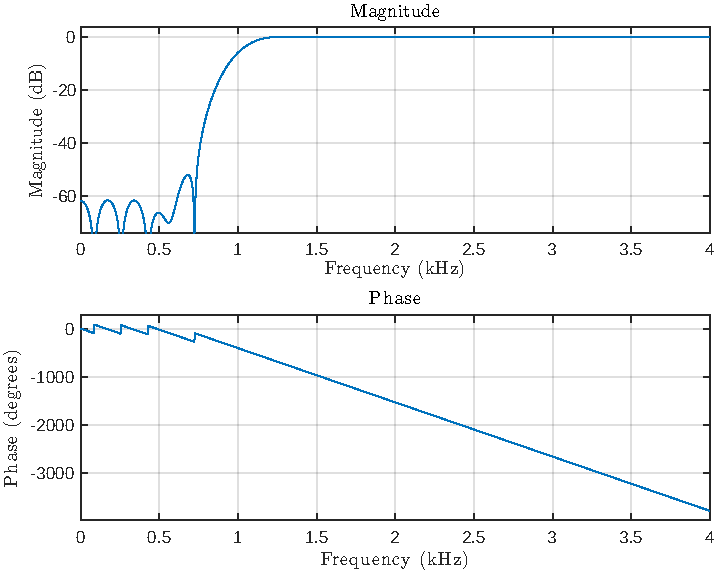
\includegraphics[width=0.75\textwidth]{figures/high-pass-fir-filter.pdf}
  \caption{Frequency Response of FIR High-Pass Filter}
\end{figure}       

\newpage
\section{Implementation and Analysis}

\subsection{Low-Pass FIR Filter on a Sinusoidal Signal with Noise}

\begin{minted}[
  frame=single,
  bgcolor=gray!10!white,
  linenos,
  ]{matlab}
% Design a low-pass filter with a cutoff frequency of 1000 Hz
% Apply the filter to a sinusoidal signals with added noise
% Plot the original signal and the filtered signal
Fs = 48000;     % Sampling frequency in Hz
Fc = 1000;      % Cutoff frequency in Hz
N = 100;        % Filter order
ftype = "low";  % Filter type

Fc_norm = Fc / (Fs/2);        % Normalize the cutoff frequency
h = fir1(N, Fc_norm, ftype);  % Design the filter

% Generate a sinusoidal signal with added noise
t = 0:1/Fs:1;
x = sin(2*pi*1000*t) + 0.5*randn(size(t));

% Apply the filter to the signal
y = filter(h, 1, x);

% Plot the original signal and the filtered signal
figure;
subplot(2,1,1);
plot(t, x);
title('Original Signal');
xlabel('Time (s)');
ylabel('Amplitude');
grid on;

subplot(2,1,2);
plot(t, y);
title('Filtered Signal');
xlabel('Time (s)');
ylabel('Amplitude');
grid on;

zoom xon;
zoom(100);
\end{minted}

In this code snippet, the cutoff frequency is set to 1000 Hz so that it
matches our desired frequency of the sinusoidal signal \( \sin (2\pi \cdot
1\text{k} \cdot t) \). The filter is then applied to the sinusoidal signal
with added noise to demonstrate the filtering effect.

\begin{figure}[hb]
  \begin{center}
    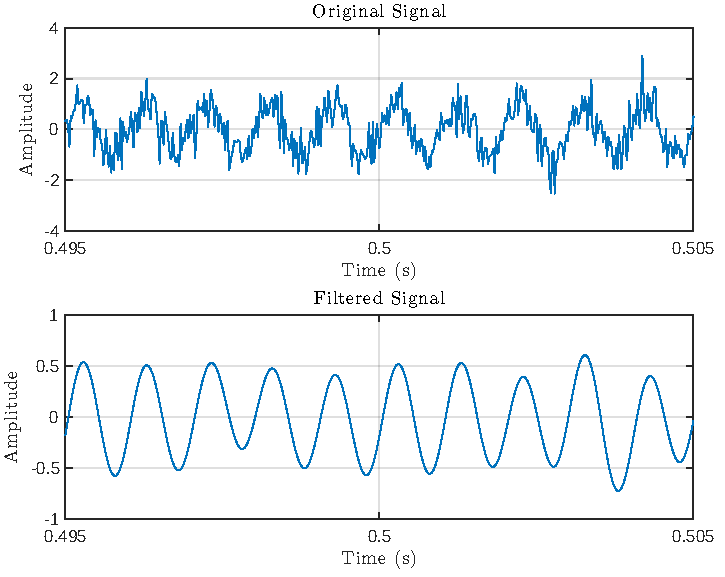
\includegraphics[width=\textwidth]{figures/low-pass-fir-filter-on-sin-wave.pdf}
  \end{center}
  \caption{Low-Pass FIR Filter Applied to a Sinusoidal Signal with Noise}
\end{figure}

\newpage

\subsection{High-Pass FIR Filter on a Composite Sinusoidal Signal}
    
\begin{minted}[
  frame=single,
  bgcolor=gray!10!white,
  linenos,
]{matlab}
% Design a high-pass filter with a passband frequency of 1500 Hz
% Apply the filter to a composite sinusoidal signal
% Plot the original signal and the filtered signal
Fs = 48000;     % Sampling frequency in Hz
Fp = 1500;      % Passband frequency in Hz
N = 100;        % Filter order
ftype = "high"; % Filter type

Fp_norm = Fp / (Fs/2);        % Normalize the passband frequency
h = fir1(N, Fp_norm, ftype);  % Design the filter

% Generate a composite sinusoidal signal
t = 0:1/Fs:1;
x = sin(2*pi*1000*t) + sin(2*pi*2000*t);

% Apply the filter to the signal
y = filter(h, 1, x);

% Plot the original signal and the filtered signal
figure;
subplot(2,1,1);
plot(t, x);
title('Original Signal');
xlabel('Time (s)');
ylabel('Amplitude');
grid on;

subplot(2,1,2);
plot(t, y);
title('Filtered Signal');
xlabel('Time (s)');
ylabel('Amplitude');
grid on;

zoom xon;
zoom(100);
\end{minted}

In this code snippet, the passband frequency is set to 1500 Hz so that the
composite sinusoidal wave of \( \sin (2\pi \cdot 1\text{k} \cdot t) + \sin
(2\pi \cdot 2\text{k} \cdot t) \) get filtered into the higher frequency
component of 2 kHz.

\begin{figure}[p]
  \begin{center}
    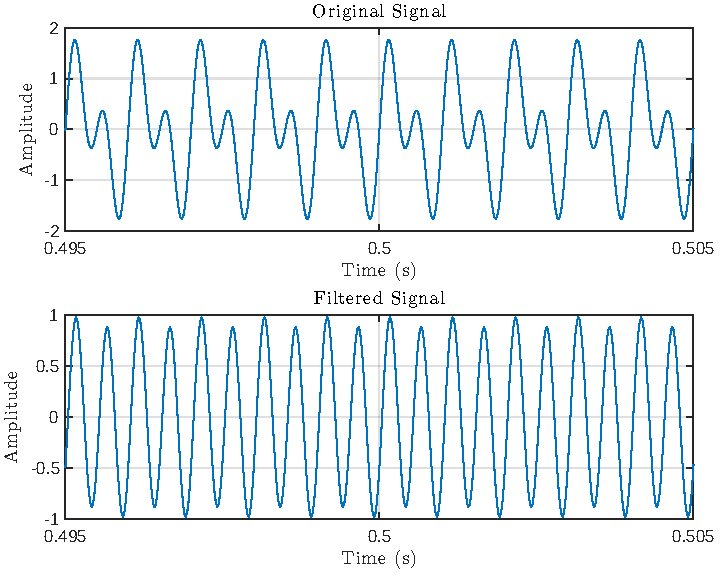
\includegraphics[width=\textwidth]{figures/high-pass-fir-filter-on-sin-wave.pdf}
  \end{center}
  \caption{High-Pass FIR Filter Applied to a Composite Sinusoidal Signal}
\end{figure}

\newpage

\section{Conceptual Understanding}
\subsection{Low-pass Filter}
For a simple first-order low-pass filter
\begin{equation}
  H(s) = \frac{1}{1 + s/\omega_c},
\end{equation}
where \(s\) is the complex frequency variable, and \(\omega_c\) is the
cutoff frequency. The transfer function \(H(s)\) describes the
relationship between the input and output signals of the filter.
\begin{figure}[h]
  \centering
  \begin{tikzpicture}[american,thick]

    % Change components size
    \ctikzset{
      resistors/scale=0.8,
      capacitors/scale=0.7,
    }

    % Circuit code
    \draw (0,0) to[short,*-*] ++ (4,0);
    \draw (0,2) to[R=R,*-] ++ (3,0) coordinate(a);
    \draw (a) to[short,-*] ++ (1,0);
    \draw (a) to[C,l_=C,*-*] ++(0,-2);

    % Voltage labels
    \draw (0,2) to[open,v=V$_{in}$] ++(0,-2);
    \draw (4,2) to[open,v=V$_{out}$] ++(0,-2);

  \end{tikzpicture}
  \caption{RC Low-Pass Filter}
\end{figure}

The input signal $V_{\text{in}}$ is applied across the series combination of
the resistor $R$ and the capacitor $C$. Since the resistor $R$ and the
capacitor $C$ are in series, they form a voltage divider network. The voltage
across the capacitor ($V_{\text{out}}$) is the output of the low-pass filter. 

At low frequencies, the capacitive reactance $X_c$ of the capacitor is high,
meaning it acts like an open circuit and allows most of the input signal to
pass through to the output $V_{\text{out}}$. The impedance $Z$ of a capacitor
is given by the formula $Z = \frac{1}{j\omega C}$, where \(  \) is the
imaginary unit, ω is the angular frequency \( 2\pi f \), and $C$ is the
capacitance.

As the frequency of the input signal increases, the capacitive reactance ($X_{c}$)
decreases inversely proportional to frequency $Xc = \frac{1}{2πfC}$. When the
frequency reaches a certain point known as the cutoff frequency $f_C$, the
capacitive reactance becomes comparable to the resistance in the
circuit.

At frequencies below the cutoff frequency ($f < f_C$), the capacitor effectively
blocks the higher-frequency components of the input signal, allowing primarily
the lower-frequency components to pass through to the output. This filtering
action is due to the high impedance of the capacitor at lower frequencies.

As the frequency of the input signal exceeds the cutoff frequency ($f>f_C$), the
capacitive reactance ($X_c$) decreases, and more signal is diverted through the
capacitor to ground rather than passing through to the output. This results in
attenuation of higher frequencies, effectively filtering them out from the
output.


        

\subsection{High-pass Filter:} 

For a simple first-order high-pass filter

\begin{equation}
  H(s) = \frac{s}{s + \omega_c},
\end{equation}
\begin{figure}[h]
  \centering
  \begin{tikzpicture}[american,thick]

    % Change components size
    \ctikzset{
      resistors/scale=0.8,
      capacitors/scale=0.7,
    }

    % Circuit code
    \draw (0,0) to[short,*-*] ++ (4,0);
    \draw (0,2) to[C=C,*-] ++ (3,0) coordinate(a);
    \draw (a) to[short,-*] ++ (1,0);
    \draw (a) to[R,l_=R,*-*] ++(0,-2);

    % Voltage labels
    \draw (0,2) to[open,v=V$_{in}$] ++(0,-2);
    \draw (4,2) to[open,v=V$_{out}$] ++(0,-2);

  \end{tikzpicture}
  \caption{RC High-Pass Filter}
\end{figure}

The input signal $V_{\text{in}}$ is applied across the series combination of
the capacitor $C$ and the resistor $R$. Since the capacitor $C$ and the resistor
$R$ are in series, they form a voltage divider network. The voltage across the
resistor ($V_{\text{out}}$) is the output of the high-pass filter.

At low frequencies, the capacitive reactance $X_c$ of the capacitor is high,
meaning it acts like an open circuit and allows most of the input signal to
pass through to the output $V_{\text{out}}$. The impedance $Z$ of a capacitor
is given by the formula $Z = \frac{1}{j\omega C}$, where $j$ is the imaginary
unit, ω is the angular frequency \(2\pi f\), and $C$ is the capacitance.

As the frequency of the input signal increases, the capacitive reactance ($X_{c}$)
decreases inversely proportional to frequency $X_{c} = \frac{1}{2\pi fC}$. When
the frequency reaches a certain point known as the cutoff frequency $f_C$, the
capacitive reactance becomes comparable to the resistance in the circuit.

At frequencies below the cutoff frequency ($f < f_C$), the capacitor effectively
blocks the lower-frequency components of the input signal, allowing primarily
the higher-frequency components to pass through to the output. This filtering
action is due to the high impedance of the capacitor at lower frequencies.

As the frequency of the input signal exceeds the cutoff frequency ($f > f_C$), the
capacitive reactance ($X_c$) decreases, and more signal is diverted through the
capacitor to ground rather than passing through to the output. This results in
attenuation of lower frequencies, effectively filtering them out from the output.

\subsection{Trade-offs in Filter Design}

\begin{enumerate}
  \item \textbf{Filter Order:} The order of a filter refers to the number of
    reactive components (capacitors or inductors) in the filter design.
    Higher-order filters have steeper roll-off characteristics, meaning they
    can achieve sharper transitions between passbands and stopbands. However,
    increasing the filter order also increases complexity and introduces more
    components, leading to higher cost and potential signal distortion.
  \item \textbf{Frequency Selectivity:} Frequency selectivity refers to how
    well a filter can discriminate between desired signal frequencies and
    unwanted frequencies. Higher-order filters generally offer better frequency
    selectivity by providing narrower passbands and deeper stopbands. However,
    this increased selectivity often comes at the expense of wider transition
    bands and higher latency.
  \item \textbf{Passband Ripple:} Passband ripple refers to the variation in
    gain within the passband of a filter. Lower passband ripple indicates a
    more consistent gain across the passband, resulting in less distortion of
    the desired signal. However, achieving lower passband ripple may require
    more complex filter designs or higher-order filters.
  \item \textbf{Attenuation:} Attenuation denotes how effectively a filter
    suppresses frequencies outside its passband. Higher attenuation levels are
    crucial for applications where noise or interference must be minimized.
    However, achieving higher attenuation may require sacrificing passband
    flatness or introducing more components.
  \item \textbf{Phase Response:} Filters can introduce phase shifts to the
    signals passing through them, affecting the timing relationships within the
    signal. Linear phase filters maintain constant group delay across all
    frequencies, preserving signal integrity but often at the cost of increased
    complexity.
  \item \textbf{Group Delay:} Group delay measures the time delay experienced
    by different frequency components of a signal. For real-time applications,
    minimizing group delay is essential to prevent signal distortion and
    maintain fidelity.
\end{enumerate}

\section{Nosiy ECG Signal (Bonus)}
Used data from the PhysioNet MIT-BIH Noise Stress Test Database
\cite{goldberger2000physiobank}, the ECG signal was recorded at a sampling
frequency of 360 Hz. The signal was corrupted with a signal-to-noise ratio
(SNR) of 12 dB. The cutoff and passband frequencies were set to 5 Hz and 20 Hz,
respectively, with a filter order of 1001 taps \cite{marchon2019efficient}.

\begin{minted}[
  frame=single,
  bgcolor=gray!10!white,
  linenos,
]{matlab}
Fs = 360; % Sampling frequency in Hz
Fp = 5; % Passband frequency in Hz
Fc = 20; % Cutoff frequency in Hz
N = 1001;   % Filter order

Fp_norm = Fp / (Fs/2);        % Normalize the passband frequency
Fc_norm = Fc / (Fs/2);        % Normalize the cutoff frequency
h = fir1(N, [Fp_norm Fc_norm]); % Generate the filter coefficients

% Read the ECG signal
% The ECG signal is stored in a CSV file with one column
% The sampling frequency is 360 Hz
ecg = csvread('118e12.csv');

% Apply the filter to the ECG signal
filtered_ecg = filter(h, 1, ecg);

% Plot the original and filtered ECG signals
figure;
subplot(2,1,1);
plot(ecg);
title('Original ECG Signal');
xlim([1000 2000]);
ylim([-8 -4]);
grid on;

subplot(2,1,2);
plot(filtered_ecg);
title('Filtered ECG Signal');
xlim([1000 2000]);
ylim([-1 1]);
grid on;
\end{minted}

\begin{figure}[p]
  \centering
  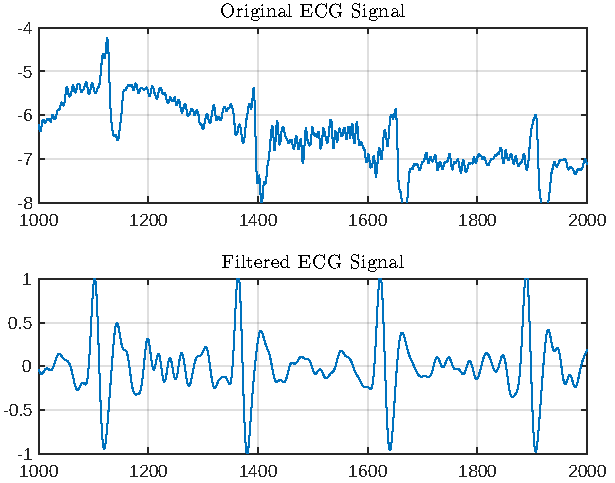
\includegraphics[width=\textwidth]{figures/ecg-signal.pdf}
  \caption{ECG Signals of Heartbeat}
\end{figure}

\newpage
\printbibliography[heading=bibnumbered]

\end{document}
